\chapter{Anexo I: Matriz de Consistencia}

\begin{table}[htbp]
\centering
\small
\begin{tabular}{|p{5cm}|p{5cm}|p{5cm}|}
\hline
\textbf{Problema} & \textbf{Objetivos} & \textbf{Hipótesis} \\
\hline
¿De qué manera una aplicación móvil mediante el uso de inteligencia artificial generativa puede contribuir al control, monitoreo integral y educación de los pacientes con cáncer de mama? 
& Desarrollar una aplicación móvil basada en Inteligencia Artificial generativa para el monitoreo integral y el control de pacientes con cáncer, que mejore la adherencia al tratamiento, el seguimiento de signos vitales, el soporte emocional y conocimiento sobre la enfermedad. 
& El desarrollo de una aplicación móvil que emplea Inteligencia Artificial generativa mejorará significativamente el monitoreo integral, el control y la educación de los pacientes con cáncer de mama. \\
\hline
\end{tabular}
\caption{Desarrollo de una aplicación móvil: Problema Principal, Objetivo y Hipótesis}
\label{tabla_principal}
\end{table}

\begin{table}[htbp]
\centering
\small
\begin{tabular}{|p{5cm}|p{5cm}|p{5cm}|}
\hline
\textbf{Problema específico} & \textbf{Objetivo específico} & \textbf{Hipótesis específica} \\
\hline
¿Qué base de datos se deben usar para entrenar el modelo de IA para ofrecer respuestas óptimas? 
& Identificar las bases de datos especializadas que se pueden integrar para entrenar el modelo de IA generativa de la aplicación móvil. 
& La implementación de un modelo de IA generativa entrenado con bases de datos médicas especializadas en el cáncer de mama permitirá a la aplicación móvil proporcionar respuestas precisas y personalizadas a las consultas de los pacientes, mejorando su comprensión de la enfermedad y el tratamiento. \\
\hline
¿De qué manera una aplicación móvil puede proporcionar soporte emocional a los pacientes oncológicos? 
& Implementar un sistema de IA generativa que proporcione soporte emocional personalizado en función del estado anímico del paciente. 
& La implementación de un sistema de soporte emocional automatizado mejorará el bienestar emocional de los pacientes, reduciendo su ansiedad y mejorando su calidad de vida. \\
\hline
¿Qué funcionalidades de una aplicación móvil son esenciales para el monitoreo de signos vitales en pacientes con cáncer? 
& Desarrollar un sistema de monitoreo de signos vitales en tiempo real que notifique a los pacientes sobre anomalías. 
& La integración de un sistema de monitoreo de signos vitales basado en IA reducirá las complicaciones relacionadas con la falta de detección temprana de problemas. \\
\hline
¿Cómo puede una aplicación móvil proporcionar información personalizada y actualizada sobre el cáncer de mama utilizando IA generativa? 
& Desarrollar una funcionalidad que permita a los pacientes recibir información personalizada y actualizada sobre su condición. 
& La implementación de un sistema que proporcione información personalizada mejorará el conocimiento del paciente sobre su enfermedad y su tratamiento. \\
\hline
¿Qué modelo de IA generativa se va a implementar para que las funciones de la aplicación móvil funcionen correctamente? 
& Seleccionar y optimizar el modelo de IA generativa más adecuado para integrar todas las funciones de la aplicación móvil de manera eficiente. 
& La implementación de un modelo de IA generativa optimizado permitirá que todas las funciones de la aplicación móvil (soporte emocional, monitoreo de signos vitales, información personalizada) funcionen de manera eficiente y precisa. \\
\hline
\end{tabular}
\caption{Desarrollo de una aplicación móvil: Problemas Específicos, Objetivos y Hipótesis}
\label{tabla_especificos}
\end{table}

\chapter{Anexo II: Árbol de problemas y de objetivos}

\begin{figure}[ht]
	\centering
	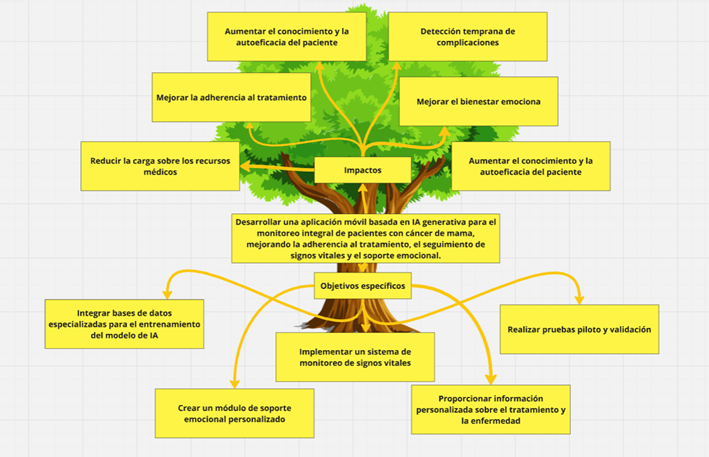
\includegraphics[width=1.1\textwidth]{anexos/Imagen1.png}
	\caption{Árbol de problemas}
	\label{8:fig}
\end{figure}

\begin{figure}[ht]
	\centering
	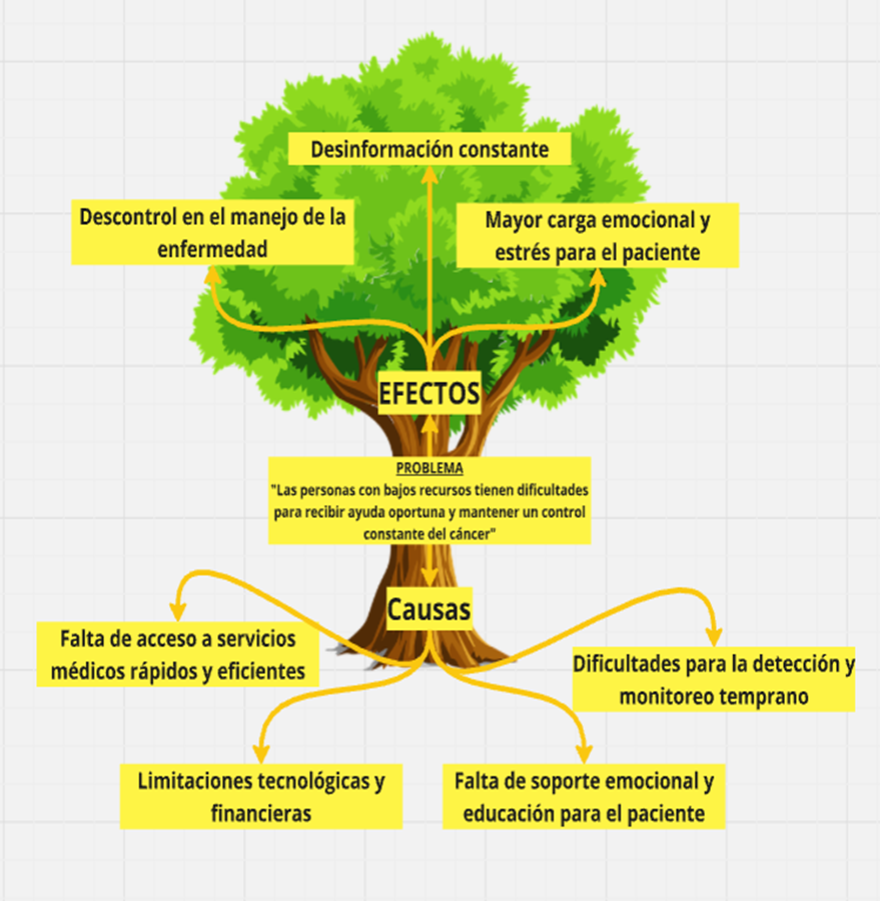
\includegraphics[width=1.1\textwidth]{anexos/Imagen2.png}
	\caption{Árbol de objetivos}
	\label{8:fig}
\end{figure}

